\glspl{MSR} are one of six advanced reactor designs shortlisted by
the \gls{GIF} in 2001 for promising significant advances in safety,
sustainability, efficiency, and cost over existing designs in operation
today. This has attracted significant attention and resources towards
\gls{MSR} research, most noticeable by the number of start-up companies that
have emerged in recent years touting various \gls{MSR} designs. This chapter
provides a brief history of \glspl{MSR}, followed by the distinctive features
that earned the concept the label of being a Generation IV reactor. Lastly,
we present the reference specifications of the \gls{MSFR} concept studied in
this work.

\section{History}

The first \gls{MSR}, named the \gls{ARE}, dates back to the 1940s,
as part of the US Aircraft Nuclear Propulsion program
\cite{rosenthal_molten-salt_1970}; the molten salt concept was considered due
to the stability of molten salts at high temperatures and neutron radiation.
The 2.5 MW$_{\text{th}}$ reactor was built at \gls{ORNL}, where it achieved
criticality on November 1954 and generated 100 MWh over nine days
\cite{rosenthal_molten-salt_1970}. The fuel
consisted of enriched uranium in a molten salt mixture of NaF, ZrF$_4$, and
UF$_4$, and moderated by blocks of beryllium oxide. The project ultimately
never came to fruition as the development of intercontinental ballistic
missiles effectively eliminated the need for long-range nuclear-powered
bomber aircraft.

However, the successful demonstration of the \gls{ARE} spurred further
research into adapting \glspl{MSR} for civilian power generation
\cite{rosenthal_molten-salt_1970}. One of the key findings from the
research was that better economy could be achieved from breeding $^{233}$U
from $^{232}$Th in thermal-spectrum reactors than $^{239}$Pu from $^{238}$U
\cite{macpherson_molten_1985}. Ultimately, these efforts culminated in the
design, construction, and successful operation of the \gls{MSRE}, a graphite
moderated thermal \gls{MSR}. Although no breeding was attempted with the
\gls{MSRE}, scientists at \gls{ORNL} obtained a wealth of experimental data
and new insights from the study of this reactor. The \gls{MSRE} had a
graphite-moderated design with LiF-BeF$_2$-ZrF$_4$-UF$_4$ fuel salt mixture,
initially rated at 10 MW$_{\text{th}}$ but later restricted to 8 M
$_{\text{th}}$ due to a miscalculation of heat transfer capabilities
\cite{haubenreich_experience_1970}. 

Design of the \gls{MSRE} commenced in the summer of 1960, with construction
starting in early 1962 \cite{haubenreich_experience_1970}. The reactor
achieved zero-power criticality in June 1965, and 30 days of continuous
operation at full power in December 1966. The reactor operated at full power
for the most of the following 15 months, during which the researchers carried
out various experiments. Soon after shutdown, the $^{235}$U fuel was replaced
with $^{233}$U and in January 1969, the \gls{MSRE} became the first reactor to
run on $^{233}$U fuel. Further experiments were run, including xenon
stripping, fission product deposition, tritium behavior, and plutonium
addition studies, before the \gls{MSRE} was permanently shut down to conserve
remaining funding for other related activities \cite{macpherson_molten_1985}.

Building on the \gls{MSRE}'s hugely successful run, \gls{ORNL} proposed a
major development project for the construction and operation of the
\gls{MSBR} \cite{macpherson_molten_1985}. However, they failed to secure
funding on two separate occasions in 1972 and 1974; they lost out to the
competing \gls{LMFBR} program which had a head start and wider
political and technical support. Nevertheless, from a technical perspective,
two independent technology evaluation and design studies of the \gls{MSR} had
``reported favorably on the promise of the system''
\cite{macpherson_molten_1985}.



\section{Features}

As mentioned in the introduction section, the most significant difference
between \glspl{MSR} and other reactor
concepts is the liquid fuel in \glspl{MSR}; fissile and/or fertile material
is dissolved in
high temperature, commonly eutectic mixtures of molten salts. Most \gls{MSR}
designs are circulating-fuel reactors. The primary coolant loop containing
the fuel salt transfers heat through a heat exchanger to the clean,
secondary/intermediate loop.

The flexibility of \glspl{MSR} is best illustrated by the various designs
under development today. Graphite-moderated thermal-spectrum \glspl{MSR} are
typically straight-forward \gls{LEU} burners, or $^{232}$Th/$^{233}$U
breeders, while epithermal- and fast-spectrum \glspl{MSR} have the additional
options of operating as \gls{TRU} fuel burners or $^{238}$U/$^{239}$Pu
breeders. Breeder designs can be further categorized into one- or two-fluid
designs; two-fluid designs feature blanket molten salt mixtures that contain
higher proportions of fertile material than the fuel salt mixture.

\section{Molten Salt Fast Reactor}

The \gls{MSFR} is a reference fast-spectrum \gls{MSR} concept developed
under the \gls{EVOL} and \gls{SAMOFAR} projects. The main reactor
specifications and schematic view are shown in Table \ref{table:msfr} and Fig.
\ref{fig:msfr} respectively. Inspired by the \gls{MSBR}, the \gls{MSFR} is
intended to run primarily on a closed thorium fuel cycle with
continuous online fuel reprocessing. Several reasons motivated the omission of
graphite moderators from the \gls{MSFR} design. Graphite is susceptible to
long-term radiation damage and replacement is likely to be necessary during
the operating lifetime of the reactor. The relatively fast neutron spectrum
improves breeding ratios due to higher fission neutron yield in $^{233}$U and
lower parasitic absorption in non-fuel materials. Lastly, graphite has a
positive temperature coefficient of reactivity; eliminating graphite from the
design ensures a greater safety margin.
%
\begin{figure}[htb!] 
	\centering
	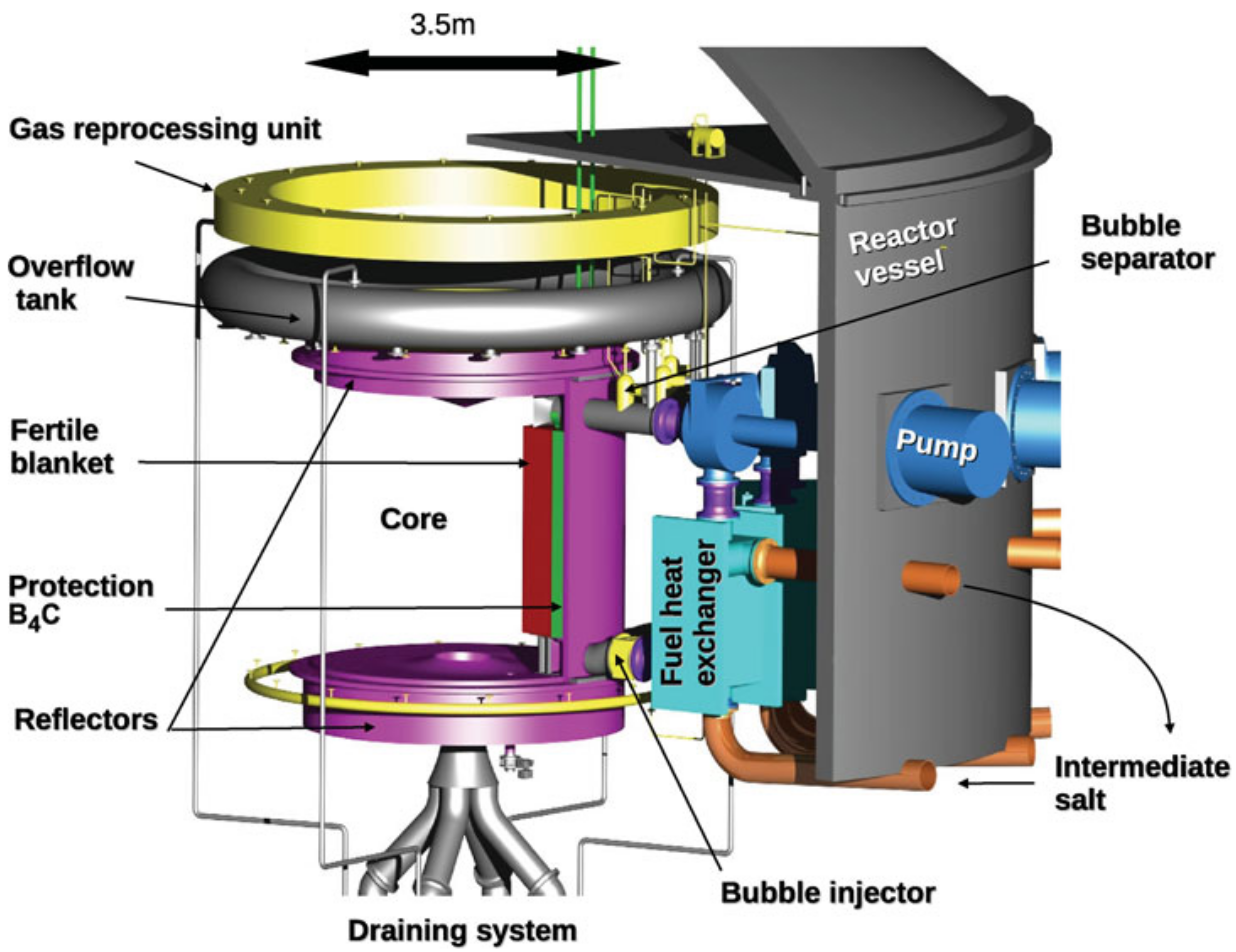
\includegraphics[width=0.6\textwidth]{MSFR}
	\caption{Schematic view of the MSFR concept \cite{serp_molten_2014}.}
	\label{fig:msfr}
\end{figure}
%
\begin{table}[htb!]
	\caption{Main specifications of the \gls{MSFR} concept
				\cite{serp_molten_2014}.}
	\centering
	\begin{tabular}{ l r }
		\hline
		Parameter & Value \\
		\hline
		Thermal/Electric output [MW$_{\text{th}}$/MW$_{\text{e}}$] & 3000 /
		1500 
		\\
		Salt volume [m$^3$] & 18 \\
		Salt fraction in core & 0.5 \\
		Number of circulation loops & 16 \\
		Nominal flow rate [kg s$^{-1}$] & 18500  \\
		Nominal circulation time [s] & 4.0 \\
		Inlet/outlet temperature [K] & 923 / 1023 \\
		Blanket volume [m$^3$] & 7.3\\
		\hline
	\end{tabular}
	\label{table:msfr}
\end{table}

In the \gls{MSFR} design, fuel salt flows upwards through a 9 m$^3$ central
core region. At the top of the core, the flow separates into 16 smaller
external loops, each of which passes through a heat exchanger before being
pumped back into the bottom of the core. Other instrumentation are situated
along the external loop for online salt reprocessing and gas sparging. The
core is surrounded axially by nickel alloy reflectors, and radially by a
toroidal blanket tank containing fertile salt for breeding. There is a layer
of boron carbide behind the blanket tanks to protect the peripheral equipment
from excessive neutron damage. In case of severe accidents, there is an
actively cooled freeze plug at the bottom of the core that melts when
temperatures exceed a certain threshold. The fuel salt would drain into a
containment vessel designed to keep it subcritical. Reactivity control under
normal operating conditions is performed by varying pump speeds to advantage
of strong thermal feedback. Coupled with the fact that there is no excess
reactivity reserve due to online fuel reprocessing, control rods are not
included in the \gls{MSFR} design.

Although the \gls{MSFR} is primarily designed to operate on the thorium fuel
cycle, it can support a range of start-up fuel and feed compositions. This
versatility is particularly important for the first few \glspl{MSFR} to be
deployed due to the lack of $^{233}$U reserves required for the initial core
loading. In general, the fuel and blanket salts are approximately composed of
eutectic mixtures of 77.5\% LiF - 22.5\% AcF$_4$, where AcF$_4$ represents
actinide fluorides such as uranium, thorium, plutonium, and other \gls{TRU}
fluorides. For an initial composition consisting of $^{232}$Th and $^{233}$U,
the benchmark value for the amount of uranium for criticality under
normal operating conditions is 2.515 mol\%. However, most code verification
studies adjust the ratio of $^{232}$Th to $^{233}$U to achieve exact
criticality at a uniform temperature of 973 K; this ensures that subsequent
neutronics and safety analyses are not affected by the difference in
k$_{\text{eff}}$ values. We performed the same exercise in this paper.

Power output of the \gls{MSFR} is rated at 3000 MW$_{\text{th}}$ and 1500
MW$_{\text{e}}$. It has a high thermal efficiency due to the high operating
temperature. \glspl{MSR} in general are not restricted by the same pressure
constraints seen in \glspl{LWR}. The inlet and outlet temperature
specifications of the fuel salt are 923 K and 1023 K respectively. This was
motivated by the need for a minimum 50 K temperature buffer between the
operating temperatures and the melting point of the salt. The \gls{MSFR} has
heat exchangers and an intermediate coolant loop to isolate the power
conversion system from the highly radioactive fuel salt. This also serves as
a layer of containment between the radioactive material and the outside
environment. The exact composition of the intermediate coolant is still under
active study and not finalized yet.

\subsection{Model Geometry}

In this thesis, we study the 2-D axisymmetric representation of the
\gls{MSFR} as shown in Fig. \ref{fig:msfrgeom}. This is the same model
geometry used in a neutronic benchmark
study of the \gls{MSFR} and the coupled analyses by Fiorina et al., Aufiero
et al., and Zhang et al. Even though this is an outdated design that had been
later optimized for better flow distribution *, the analysis results are still
valid for code verification purposes. Future efforts will adopt the optimized
hourglass-shaped design for a more realistic assessment of the \gls{MSFR}.
%
\begin{figure}[htb!] 
	\centering
	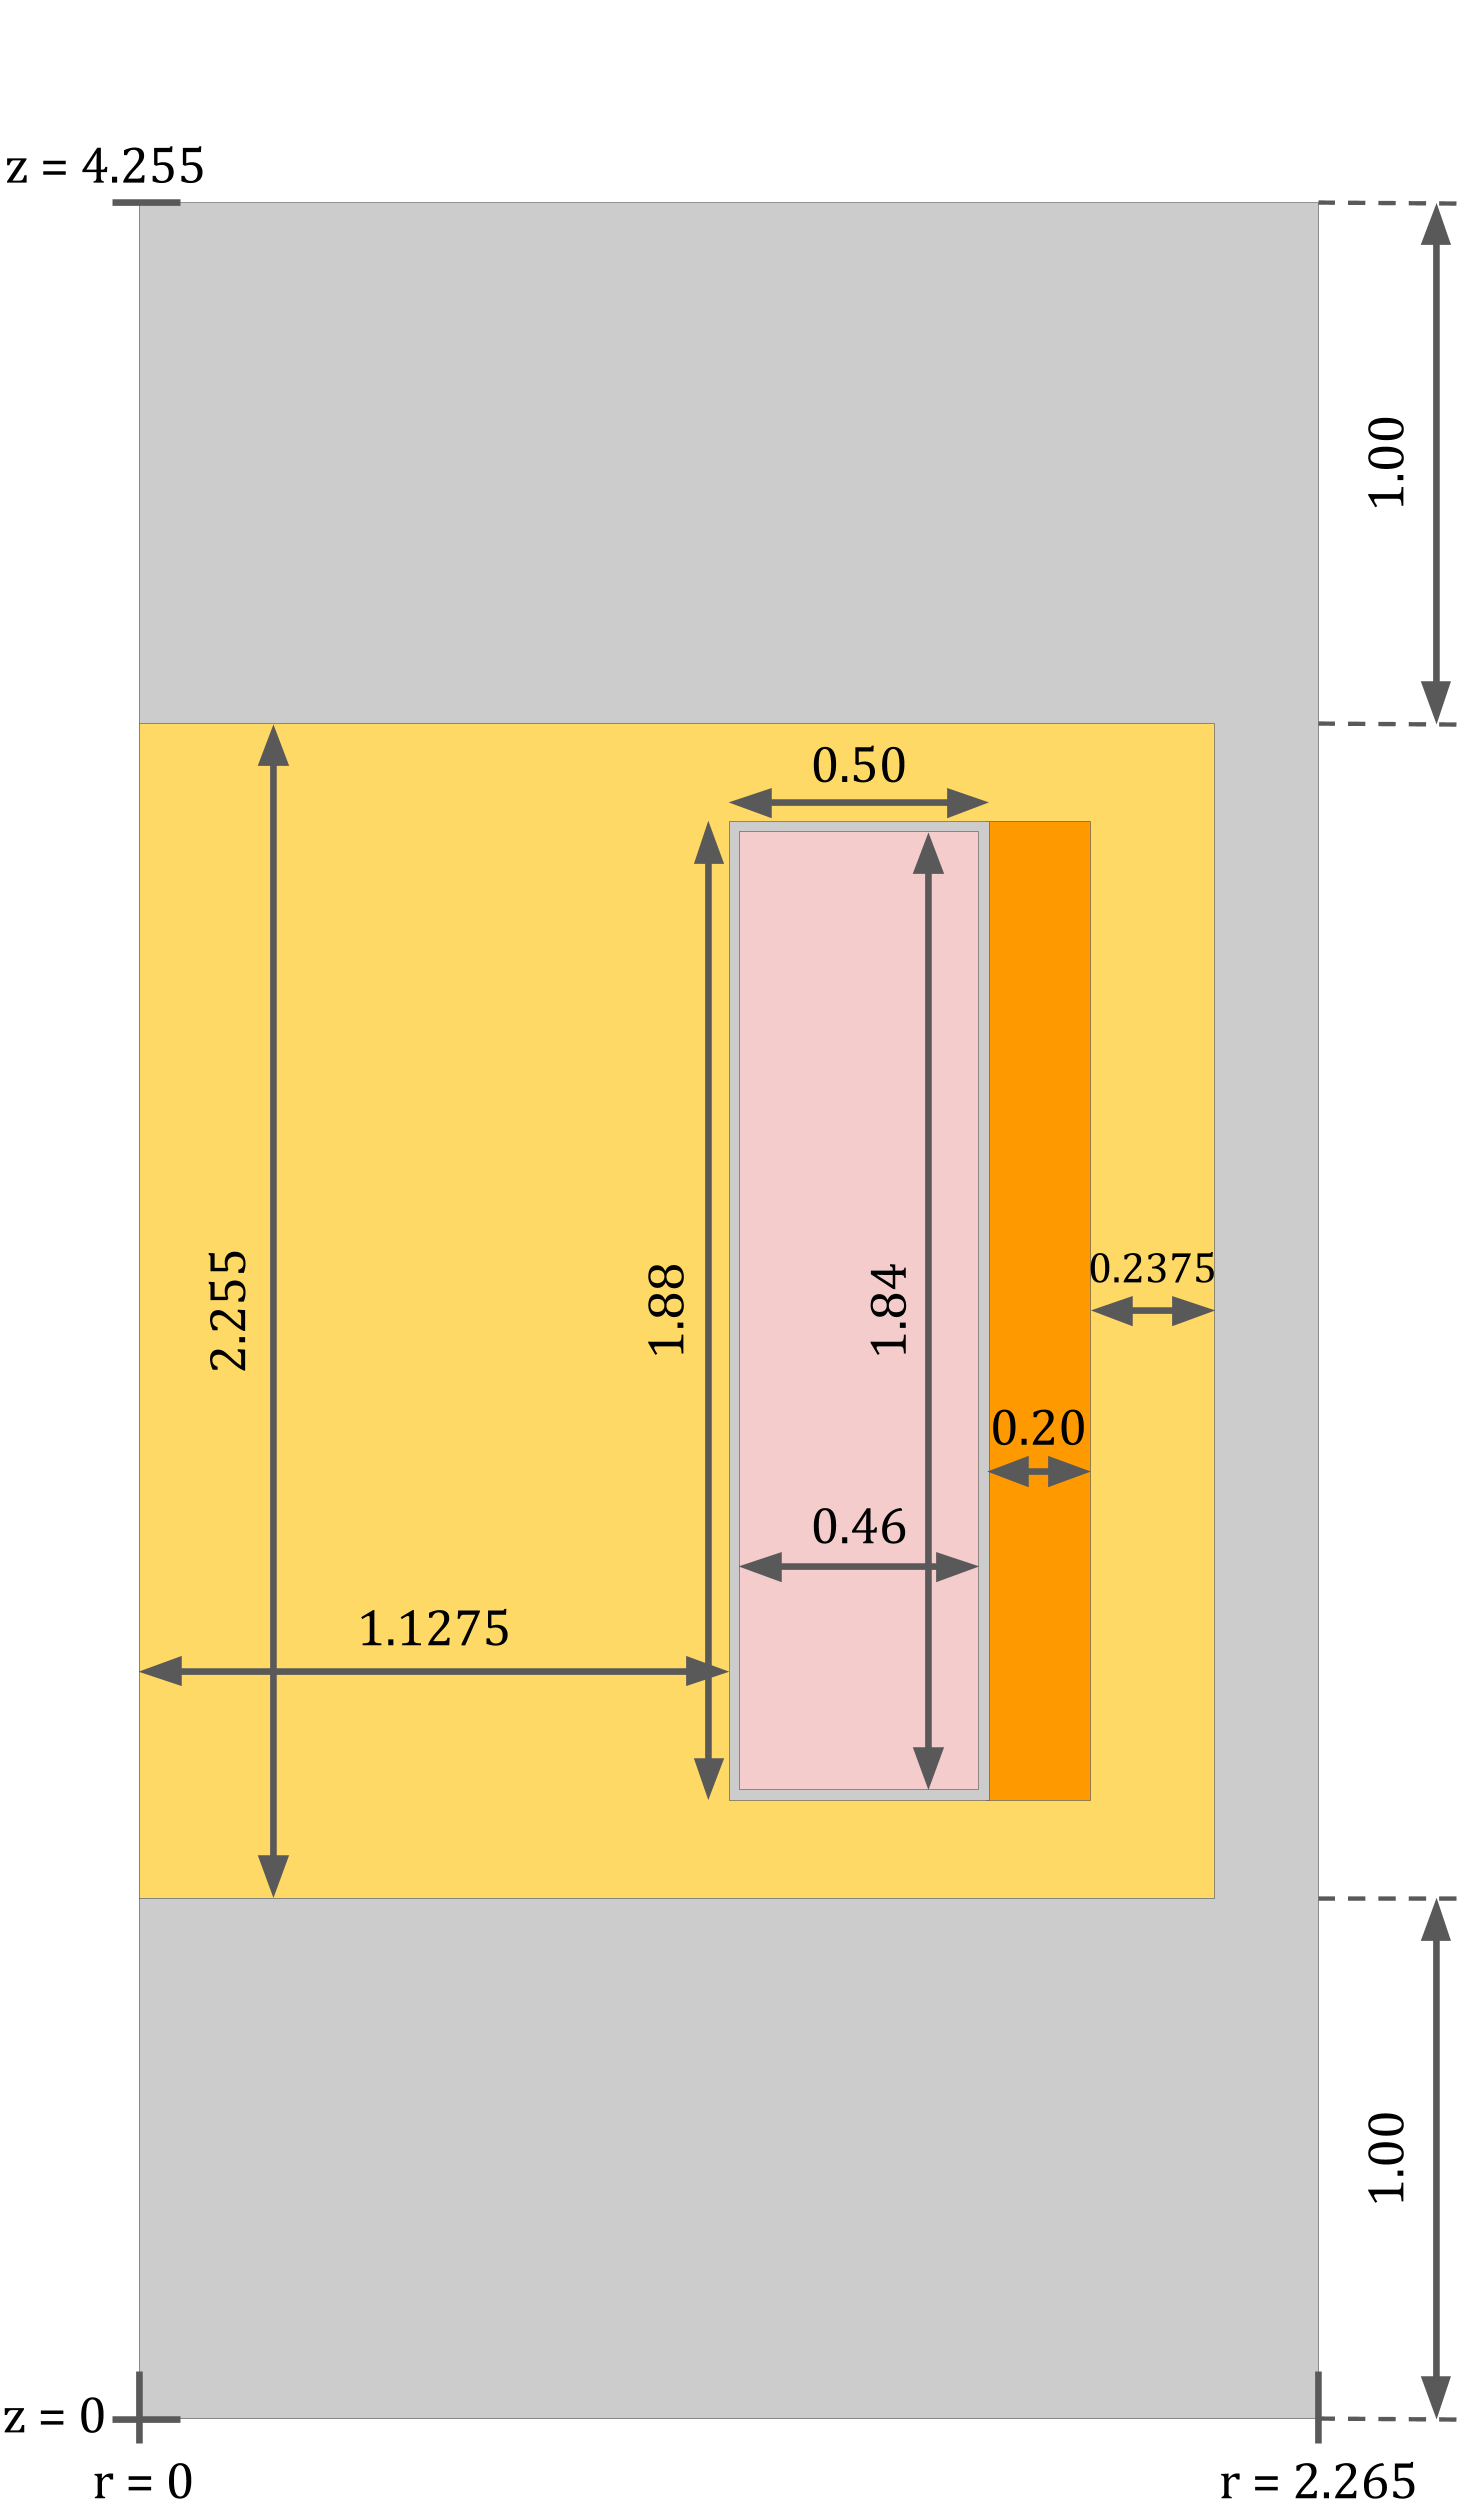
\includegraphics[width=0.5\textwidth]{msfr-geom}
	\caption{2-D axisymmetric model of the \gls{MSFR} core used for the
	simulations in Serpent and Moltres. All dimensions are in meters.
	\cite{brovchenko_neutronic_2019}}
	\label{fig:msfrgeom}
\end{figure}

For the 2-D axisymmetric model, the sixteen individual loops are homogenized
into a single loop while keeping the nominal volumetric flow rate constant.
Keeping with the model used in the previous studies, we assumed that the
region for heat exchangers and pumps on the loop consists of 100\% fuel salt.
However, this assumption has a negligible impact on the multiplication factor
due to its location behind the strong boron carbide absorber layer; 


